\chapter{Lecture 5 - Improving Rankine Cycle Performance}
\label{ch:ch5}
\section{Objectives}
The objectives of this lecture are:
\begin{itemize}
\item Describe performance parameters for Rankine Cycles
\item Illustrate benefits of Rankine Cycle with a Moisture Separator and Open Feedwater Heater
\item Show how adding a Reheater improves Performance
\item Include modeling details essential for cycle analysis
\end{itemize}

\section{Performance Changes with Increasing Steam Generator Pressure}

\newthought{Based on} our discussion from last lecture, it seems obvious enough that one way to improve Carnot efficiency and thus (hopefully!) increasing Rankine cycle performance would be to increase the steam generator temperature.  Since the steam generator is a saturated system, such a change implies an increase to steam generator pressure.  Let us assume for the time being that nothing limits us from increasing steam generator temperature and pressure; what are the thermodynamic consequences?  To start, let us examine the change on a temperature-entropy plot as is shown in Figure \ref{fig:T_S_increase_P}.

\begin{marginfigure}
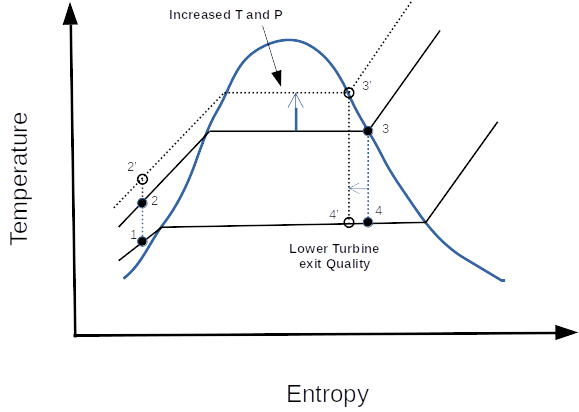
\includegraphics{T_S_increase_P.png}
\caption{Temperature Entropy plot showing an increase in steam generator pressure.}
\label{fig:T_S_increase_P}
\end{marginfigure}

\newthought{A few things} are apparent from this picture:
\begin{enumerate}
\item Since the temperature at which the majority of heat has been added to the system is increased, Carnot efficiency will increase and, all things being equal, the thermal efficiency that we actually achieve will also increase.
\item While the schematic is not drawn to scale, it suggests that net specific work will also increase at least a little. 
\item The turbine exit quality decreases after we increase the steam generator pressure.   

\end{enumerate}
The last two points on the above list might be clarified with a temperature-entropy plot that is drawn to scale.  Such a plot can be made with EasyProp tools and is shown in Figure \ref{fig:T_S_increase_P_toScale}.

\begin{marginfigure}
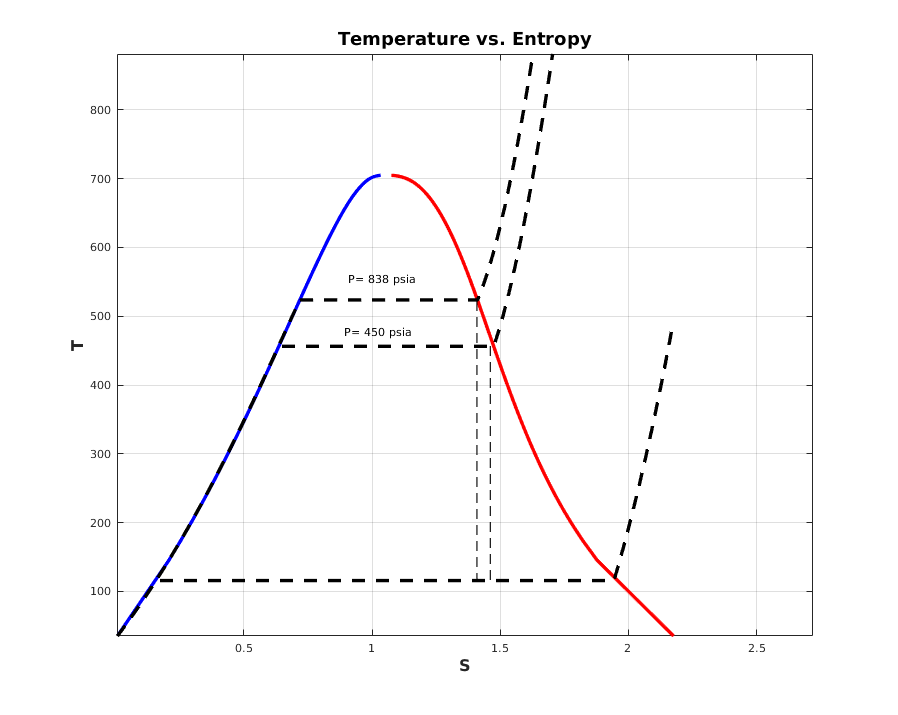
\includegraphics{TS_Pressure_Change_toScale_mf.png}
\caption{Temperature Entropy plot for steam pressure increase drawn to scale with EasyProp.}
\label{fig:T_S_increase_P_toScale}
\end{marginfigure} 

\newthought{Increasing efficiency is} a good goal but, in this case, the attendant reduction in turbine exit quality is a significant issue.  Droplets of saturated vapor in the steam can result in excessive turbine wear and reduces turbine isentropic efficiency.  The good news is that we can make changes to the cycle that address the issue with turbine exit quality while further increasing cycle thermal efficiency.

\index{Rankine Cycle, open feedwater heater}
\index{Rankine Cycle, moisture separator}
\section{Rankine Cycle with Moisture Separator and Open Feedwater Heater}
We can increase steam quality at the low-pressure stages of the turbines if, part way through the expansion process, we include a component that separates saturated liquid from the working fluid.  Such an apparatus is called a Moisture Separator (M/S) and is shown in the cycle schematic in Figure \ref{fig:RS_MS_OFWH}.

\begin{figure}
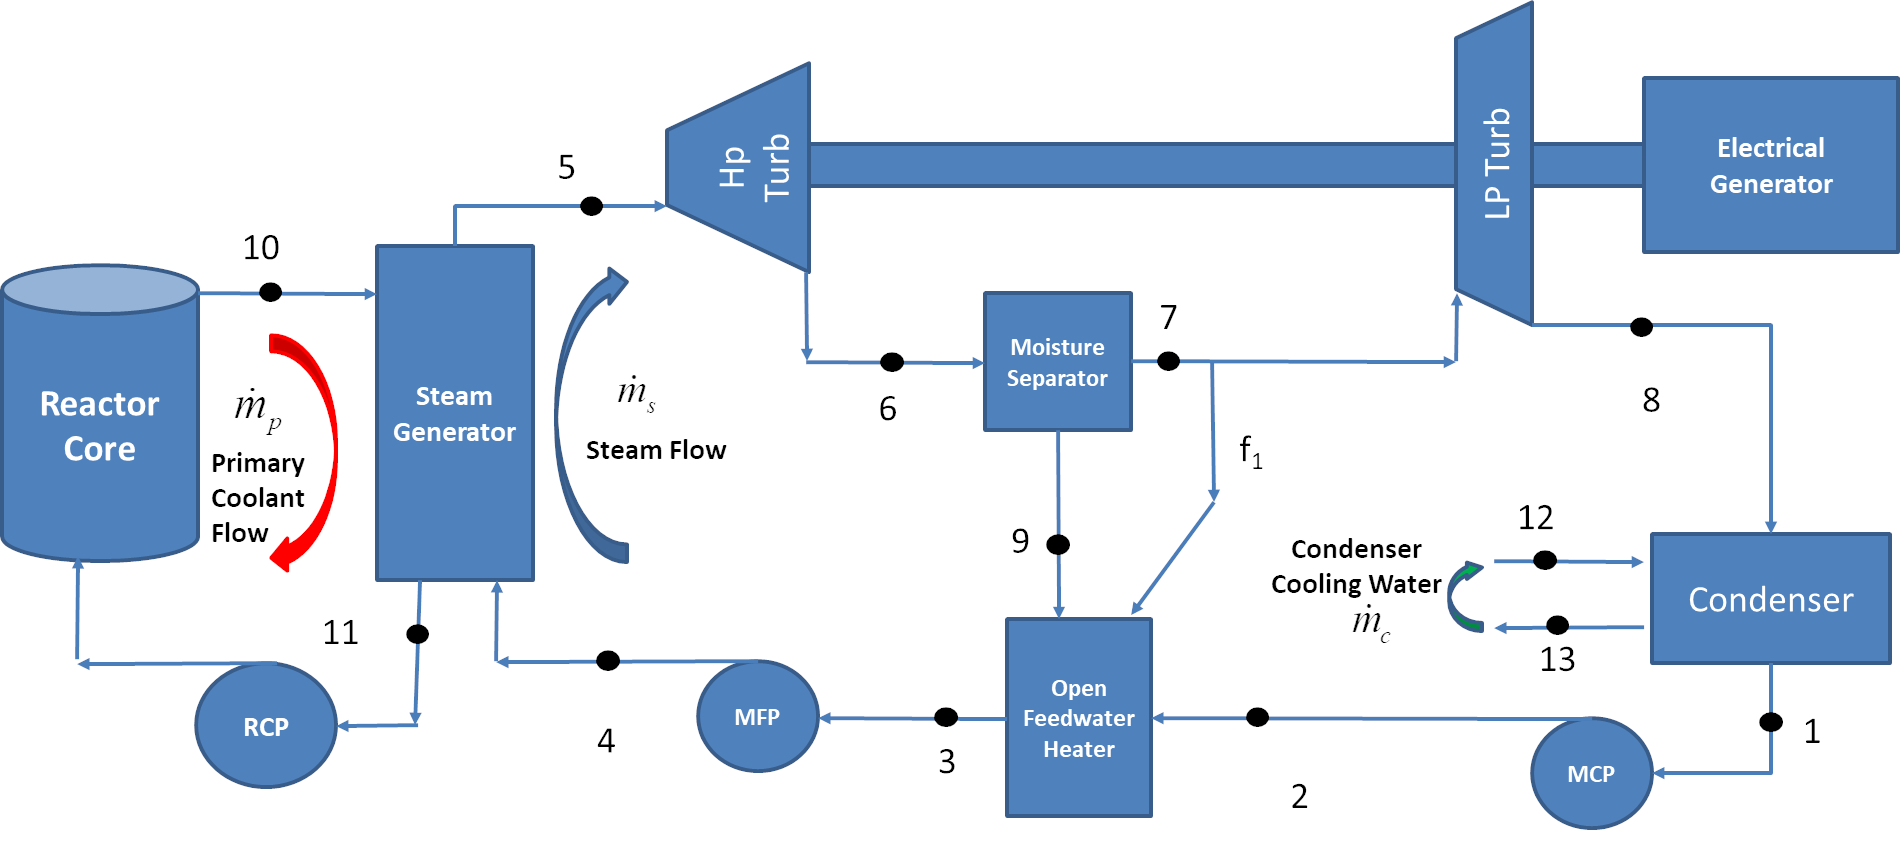
\includegraphics{Rankine_with_MS_and_OFWH.png}
\caption{Rankine Cycle with moisture separator and open feedwater heater.}
\label{fig:RS_MS_OFWH}
\end{figure} 

The moisture separator takes steam exiting the high pressure (HP) turbine at state point 6 which is a saturated mixture.  The portion of the steam that is saturated vapor\sidenote[][-1.0cm]{This fraction is easily obtained as the quality at state point 6, $x(6)$, using EasyProp.} exits the moisture separator to state point 7.  The portion of the steam that is saturated liquid\sidenote[][0cm]{Again, this can be found as the complement of quality at state point 6.} is drained to the Open Feedwater Heater (OFWH).\marginnote[1.25cm]{\textbf{Note: }The OFWH is ``open'' because all fluids flowing into the tank mix freely.  This has the added consequence that all fluid streams going into or out of the OFWH must be maintained at the same pressure.}

\newthought{There are three} streams going into the OFWH: discharge of the main condensate pump (state point 2); saturated liquid draining from the M/S (state point 9); and additional saturated vapor extracted from the steam flow path at the steam exit from the M/S (state point 7).  This last flow extraction is used to further pre-heat the feedwater in the OFWH.  Conventionally we set the extraction steam flow fraction ($f$) such that the fluid exiting the OFWH at state point 3 is near its saturation temperature.\sidenote[][-0.5cm]{We will adopt the modeling convention that the fraction $f$ extracted from the steam flow is set so the outflow from the OFWH is a saturated liquid.}

\newthought{The temperature-entropy plot} for this modified cycle is shown in Figure \ref{fig:TS_MS_OFWH}.  This illustrates how, at least, the problem of turbine exit quality is addressed.
\begin{marginfigure}
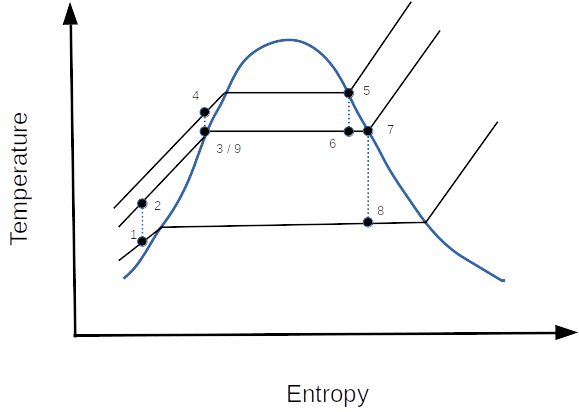
\includegraphics{TS_MS_OFWH.png}
\caption{Temperature-entropy plot of Rankine cycle with M/S and OFWH.}
\label{fig:TS_MS_OFWH}
\end{marginfigure}
One thing the figure does not show quantitatively is that the regeneration effect of pre-heating the feedwater in the OFWH has the result of increasing plant thermal efficiency.  This benefit comes at the cost of another effect that the temperature-entropy plot fails to highlight; the mass flow rate of steam through the low-pressure (LP) turbine is reduced thereby lowering specific work output from the cycle.

\subsection{``First Law'' Analysis of Modified Cycle}

\newthought{The analysis of this cycle} requires some modifications.  The reason for this is, owing to the separation of vapor and liquid in the M/S, the working fluid has different mass flow rates at different portions of the system.  For example, for a given mass flow rate through the S/G ($\dot{m}_{s}$), then the mass flow rate of steam exiting the M/S at state point 7 is $\dot{m}_s x(6)$, where $x(6)$ is the quality at state point 6.\sidenote{For this cycle where saturated vapor (x=1) is introduced into the HP turbine, $x(6)$ is generally less than 1.} Before the steam enters the LP turbine, the flow rate is further reduced since a fraction $f$ is directed to the OFWH for regeneration.  Thus the mass flow rate of steam entering the LP turbine is: $\dot{m}_s x(6)(1-f)$.

\newthought{As a convention} we will re-define ``specific work'' of a component ($w$) to be equal to the power from a component ($\dot{W}$) divided by the mass flow rate through the steam generator ($\dot{m}_s$).  See the examples below.


\begin{itemize}
%\begin{example}
\item \textbf{Example:} the specific work of the HP turbine ($w_{\text{HP}}$) is given by:
$$ w_{\text{HP}}= \frac{\dot{m}_s(h(5)-h(6))}{\dot{m}_s} = h(5) - h(6)$$
which happens to be no different than what we would have calculated before.
%\end{example}

%\begin{example}
\item \textbf{Example:} the specific work of the LP turbine ($w_{\text{LP}}$) is given by:
$$ w_{\text{LP}}= \frac{\dot{m}_s x(6) (1-f) (h(7) - h(8))}{\dot{m}_s} = x(6) (1-f) (h(7)-h(8))$$
This expression takes into account the reduced mass flow rate through the LP turbine due to the moisture separator and extraction steam.
%\end{example}

%\begin{example}
\item \textbf{Example:} the specific work of the main condensate pump (MCP) is, for this cycle, similar to the LP turbine:
$$ w_{\text{MCP}}=  \frac{\dot{m}_s x(6) (1-f) (h(1)-h(2))}{\dot{m}_s} = x(6)(1-f)(h(1)-h(2))$$
%\end{example}

%\begin{example}
\item \textbf{Example:} the specific work of the main feed pump (MFP) is:
$$ w_{\text{MFP}}= \frac{\dot{m}_s (h(3) - h(4))}{\dot{m}_s}=h(3) - h(4)$$
%\end{example}
\end{itemize}

\newthought{Use of }this convention makes calculation of net specific work easy: we simply add up the specific work of each component in the system: $w_{\text{net}} = w_{\text{HP}}+w_{\text{LP}}+w_{\text{MCP}}+w_{\text{MFP}}$.  Calculation of specific heat added is done the same way.

\newthought{Care must also} be taken for calculation of energy balances in the system.  When analyzing the simple ideal Rankine cycle, we used an energy balance on the condenser in order to determine condenser cooling water mass flow rate ($\dot{m}_{\text{c}}$).  For this cycle an equivalent analysis gives:
$$ \dot{m}_c (h(13) - h(12)) = \dot{m}_s x(6)(1-f)(h(8)-h(1))$$
Similarly, in order to deduce what the extraction steam flow fraction ($f$) must be, we will need to do an energy balance on the OFWH.  For this we will equate the rate of energy exiting the tank to the rate of energy entering the tank:
\begin{align*}
\Sigma \dot{E}_{\text{out}} &= \Sigma \dot{E}_{\text{in}} \\
\dot{m}_s h(3) &= \dot{m}_s (1-x(6))h(9) + \dot{m}_s x(6)f h(7) + \dot{m}_s x(6)(1-f)h(2)
\end{align*}\marginnote[-1cm]{\textbf{Note: }Since $\dot{m}_s$ appears in every term of the equations, it is convenient to eliminate that term from the equation.}


\section{Rankine Cycle with Reheating} \index{Rankine cycle, reheat}
We can further reduce moisture in the low-pressure sections of turbines by re-heating the steam after it exits the moisture separators.\sidenote[][-0.75cm]{In typical energy conversion cycles for commercial nuclear power plants, moisture separators and reheaters are combined into a single component called a ``moisture-separator-reheater''.}  A schematic of such a system is shown in Figure \ref{fig:RS_MS_OFWH_RH}.  
\begin{figure}
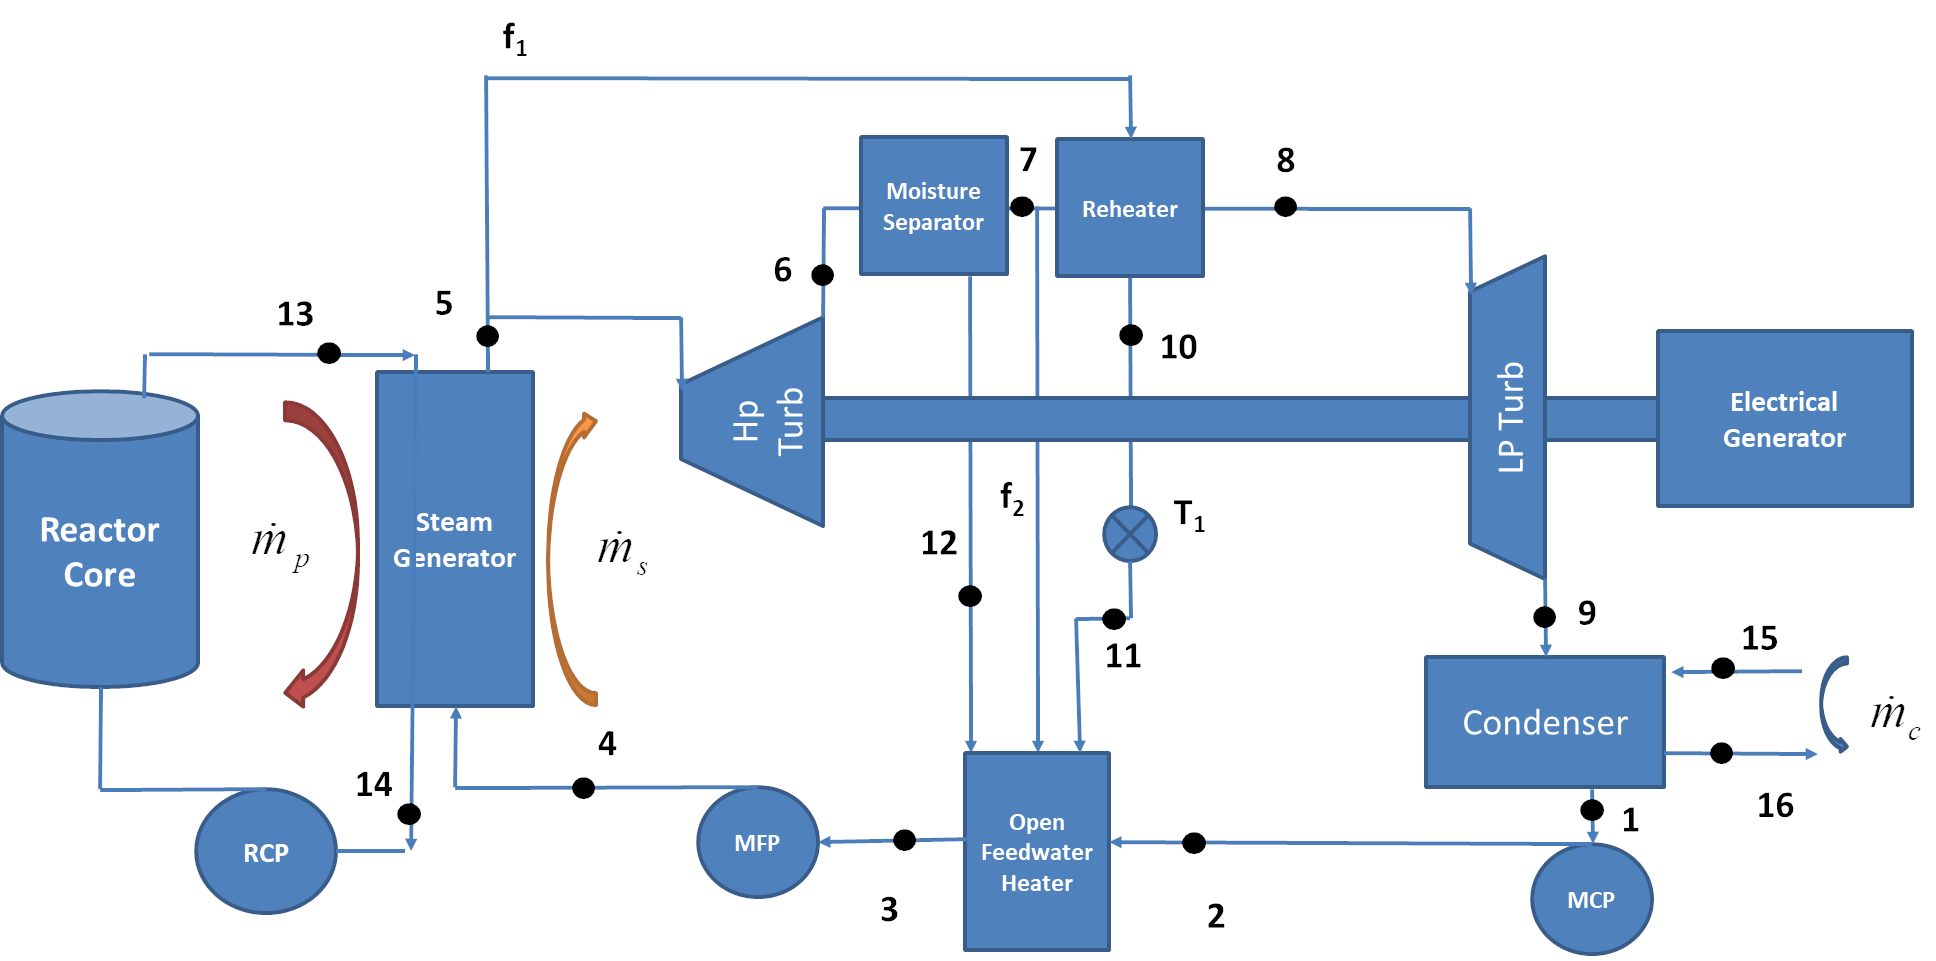
\includegraphics{Rankine_with_MS_and_OFWH_and_Reheat.png}
\caption[][0.75cm]{Rankine cycle with MS, OFWH and Reheat.}
\label{fig:RS_MS_OFWH_RH}
\end{figure}
 

The corresponding temperature-entropy sketch is provided in Figure \ref{fig:TS_MS_OFWH_RH}.  Note that the quality of the steam exiting the LP turbine at state point 9 has increased.
\begin{marginfigure}
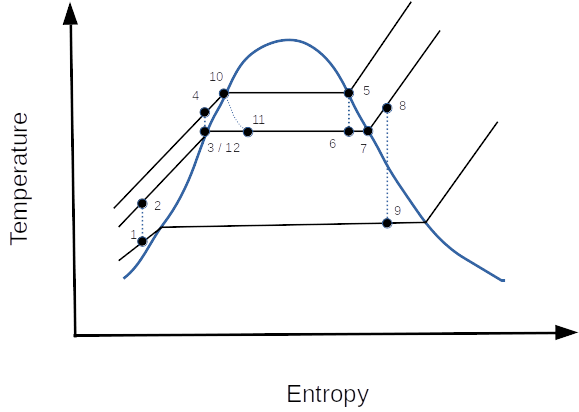
\includegraphics{TS_MS_OFWH_RH.png}
\caption{Temperature-entropy plot of modified cycle.}
\label{fig:TS_MS_OFWH_RH}
\end{marginfigure}
\newthought{There are a couple} of notable features of this cycle:
\begin{enumerate}
\item We use steam extracted upstream of the HP turbine\marginnote[0.25cm]{\textbf{Note:} Re-heat steam mass flow rate is typically around 5 percent of $\dot{m}_s$.} as the heat source to re-heat steam exiting the moisture separator. 
\item A new type of system component has been used between state points 10 and 11.  This device, which is referred to as a ``trap'' ($T_1$), allows for isenthalpic\marginnote{\textbf{Isenthalpic} means ``constant enthalpy.''} expansion of a working fluid; this is needed since the fluid at state point 10---which we will conventionally model to be in the saturated liquid state---is at higher pressure than the OFWH.  As a result of this expansion, the fluid at state point 11 will typically be a saturated mixture.
\end{enumerate}

\subsection{``First-Law'' Analysis of Modified System}
This cycle is more complicated than the last one.  We have two flow extractions ($f_1$ and $f_2$) that we need to solve for.  Consequently, we will need two equations to find a solution.  These equations will come from the energy balance for the open feedwater heater and the re-heater.  

\newthought{Using the conventions} for calculating flow fractions established in the last example, the energy balance for the OFWH is given as follows:\marginnote{\textbf{HEALTH WARNING: }you should take some time to study this equation; make sure every term makes sense and build confidence that you could derive this yourself.}
\begin{align*}
\Sigma \dot{E}_{\text{out}} &= \Sigma \dot{E}_{\text{in}} \\
\dot{m}_s h(3) &= \dot{m}_s [(1-f(1))(1-x(6))h(12) + (1-f(1))x(6)f(2)h(7)\dots \\
               & \ \ \ \ f(1)h(11) + (1-f(1))(x(6))(1-f(2))h(2) ]
\end{align*}

The energy balance for the re-heater reads as follows:
\begin{align*}
\Sigma \dot{E}_{\text{out}} &= \Sigma \dot{E}_{\text{in}} \\
\dot{m}_s(1-f(1))x(6)(1-f(2))(h(8)-h(7))&=\dot{m}_s f(1)(h(5)-h(10))
\end{align*}

Both of these equations must be solved simultaneously to find $f(1)$ and $f(2)$.  These are both non-linear equations and, for general cycle analyses, can be quite difficult to find without computational help.  In the next lecture we will discuss MATLAB tools for carrying out the required calculations.



